\chapter{Differential Equations}

A \textit{differential equation} is an equation involving a quantity and one or more of its derivatives.

\section*{1 Ordinary Differential Equations}

An ODE involves the derivative of the dependent variable with respect to a single independent variable.

\subsection{Solving by Integration}

\begin{definition}[Solution to a differential equation] A function $y = f(x)$ that satisfies the differential equation when $f$ and its derivatives are substituted into the equation.
\end{definition}

% \begin{procedure}[Making a direction field] This procedure can be used to approximately graph a differential equation, even if an explicit solution cannot be found.
  
%   Factor the equation in terms of $y' = f'(x)$. At each $x,y$-value on a grid of a graph, evaluate $y'$ and draw a short line with the slope $y'$ at the $x,y$-value.
% \end{procedure}

\begin{procedure}[Euler's Method] To numerically approximates the solution to the differential equation $y' = F(x, y)$ with $y(x_0) = y_0$,
  \[
    y_n = y_{n - 1} + F(x_{n-1}, y_{n - 1})(x_n - x_{n - 1})
  \]
\end{procedure}

\begin{definition}[Separable Equation] A separable equation is a differential equation where
  \[
    \frac{dy}{dx} = g(x)f(y)
  \]
  for some function $g(x)$ which depends only on $x$ and $f(y)$ which depends only on $y$.
\end{definition}

\begin{theorem} For a separable equation,
  \[
    \int \frac{1}{f(y)} dy = \int g(x) dx
  \]
\end{theorem}

\begin{definition}[Logistic Differential Equation] For a population $P$ which increases exponentially ($\frac{dP}{dt} \approx kP$) when the population is small compared to the carrying capacity $M$ but where the environment cannot sustain a population larger than $M$,
  \[
    \frac{dP}{dt} = kP \left(1 - \frac{P}{M}\right)
  \]
  Then
  \[
    P(t) = \frac{M}{1 + \left(\frac{M}{P_0} - 1\right)e^{-kt}}.
  \]
  and
  \[
    \frac{d^2P}{dt^2} = k^2P \left(1 - \frac{P}{M}\right) \left(1 - \frac{2P}{M}\right)
  \]
\end{definition}

\subsection{Initial-Value Problems}

\begin{definition}[Initial-Value problem]
    Assuming the function $f$ is continuous, then the function $y$ is a solution of the IVP given that
    \[
        \frac{dy}{dx} = f(x,y), y(x_0) = y_0,
    \]
    Where $x_0$ is called the \textit{initial point} for the IVP and $y_0$ is the \textit{initial value}.
\end{definition}

\subsection{Existence and Uniqueness of Solutions}

\begin{theorem}[Existence and Uniqueness]
    If $f$ is continuous, then the function $f$ as previously defined has at least one solution on the interval of continuity. If at least one solution exists and $\frac{\partial^{}f}{\partial^{}y}$ is continuous on the same interval, the solution is unique.
\end{theorem}

\subsection{Autonomous Equations}

\begin{definition}[Autonomous Equation]
    An autonomous equation is an equation where the derivative of the dependent variable can be expressed as a function of the dependent variable alone, assuming continuity.
\end{definition}

An example of an autonomous equation is

\[
    \frac{dy}{dx} = f(y) + g(x)
\]

Whereas

\[
    \frac{dy}{dx} = f(y)g(x)
\]

Is not autonomous.

Since $f(y)$ is independent of $x$, the resulting slope field has translational symmetry across the $x$-axis. A snapshot of the slope field through a vertical line $x = x_0$ is called a \textit{phase line}. A line where the direction of the slopes is indicated with arrows either going down or up is called a \textit{one-dimensional phase portrait} of the autonomous ODE.

At $y$ values where $f(y) = 0$, when the slope is zero, those points are called \textit{equilibrium points} or \textit{stationary points}.
\begin{enumerate}
    \item If surrounding solutions approach $y = y_0$ asymptomatically then the equilibrium point is \textit{asymptomatically stable} or an \textit{attractor}.
    \item If surrounding solutions move away from $y = y_0$ then the equilibrium point is \textit{unstable} or a \textit{repeller}.
    \item If surrounding solutions approach from one side and repel from another then the equilibrium point is \textit{semi-stable}.
\end{enumerate}

\subsection{Bifurcations}

A differential equation that depends on a parameter \textit{bifurcates} if there is a qualitative change in the solutions as parameter changes, meaning that the phase line changes.

We can see this change in phase line by plotting the parameter and the solution of the differential equation. The resulting graph would look like an array of phase lines. Each point on the phase lines is called a \textit{bifurcation point}.

% Issue: caption does appear
\begin{figure}[H]
    \centering
    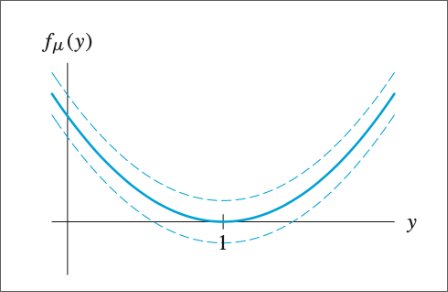
\includegraphics[width=50mm]{content/diffeq/images/bifurcation_0.png}
    \caption{Graph of $f_\mu(y) = y^2 - 2y + \mu$ for $\mu < 1$, $\mu = 1$, and $\mu > 1$.}
\end{figure}

\begin{figure}[H]
    \centering
    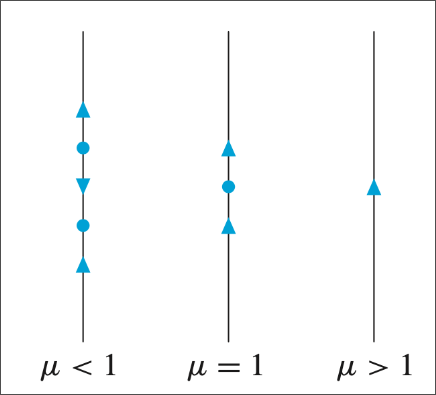
\includegraphics[width=50mm]{content/diffeq/images/bifurcation_1.png}
    \caption{Corresponding phase portraits for $\frac{dy}{dx} = y^2 - 2y + \mu$.}
\end{figure}

The typical way to visualize bifurcations is through \textit{bifurcation diagrams}. The parabola on the following figure is called a \textit{bifurcation line}.

\begin{figure}[H]
    \centering
    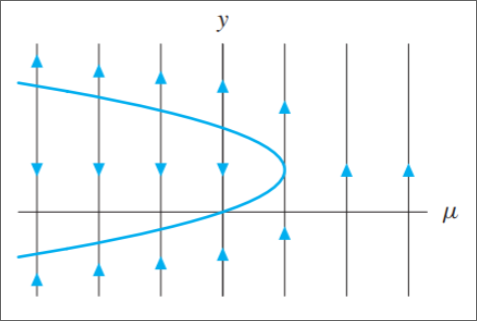
\includegraphics[width=50mm]{content/diffeq/images/bifurcation_2.png}
    \caption{Bifurcation diagram for $\frac{dy}{dx} = y^2 - 2y + \mu$.}
\end{figure}

\subsection{Separable Equations}

\begin{definition}[Separable first-order ODE]
    An ODE is separable if it can be expressed as 
    \[
        \frac{dy}{dx} = g(x)h(y)
    \]
    where $g$ and $h$ are continuous.
\end{definition}

We can simplify the process of solving a separable equations by defining the following where $H(y)$ and $G(x)$ are antiderivatives of $\frac{1}{h(y)}$ and $g(x)$, respectively, and $c \in \Real$ is an arbitrary constant.

\[
    H(y) = G(x) + c
\]

which can then be expressed as

\[
    \int \frac{1}{h(y)} dy = \int g(x) dx
\]

\subsection{Implicitly-Defined Solutions}

Sometimes a separable equation can't be solved for $y$ explicitly. Let's define $F(x,y)$ as

\[
    F(x,y) \coloneq H(y) - G(x) - c
\]

so that

\[
    F(x,y) = 0
\]

The equation above implicitly defines $y$ as a function of $x$ only if it follows the \textit{Implicit Function Theorem} from Multivariable Calculus.

\begin{theorem}[Implicit Function Theorem]
    If $F$ is defined on a disc containing $(x_0, y_0)$, where

    \begin{enumerate}
        \item $F(x,y) = 0$
        \item $\frac{\partial^{}F}{\partial^{}x}$ and $\frac{\partial^{}F}{\partial^{}y}$ are continuous on the disc
        \item $\frac{\partial^{}F}{\partial^{}x} \ne 0$
    \end{enumerate}

    then the equation $F(x,y) = 0$ defines $y$ as a function of $x$ on some open set containing the point $(x_0, y_0)$.
\end{theorem}

\subsection{Singular Solutions}

\begin{definition}[Singular Solution]
    A solution is singular if it cannot be obtained by any choice of $c$ in the solution equation of the separable ODE.
\end{definition}

When either $h(y)$ or $g(x)$ are equal to $0$ inside a separable equation, then they would be valid solutions, but may not show up in the integration method for finding solutions as defined in the Separable Equations section. If that is the case, then those solutions are unique.

\subsection{Orthogonal Trajectories}

An \textit{orthogonal trajectory} of a family of curves is a curve that intersects each curve of the family orthogonally.

\begin{figure}[H]
    \centering
    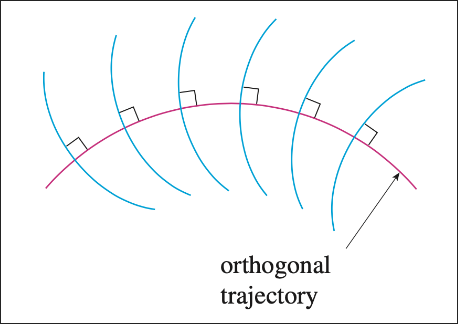
\includegraphics[width=50mm]{content/diffeq/images/orthogonal_0.png}
    \caption{An example of an orthogonal trajectory.}
\end{figure}

For example,

\[
    x^2 + y^2 = r^2
\]

and

\[
    y = mx
\]

are orthogonal trajectories of each other.

To find orthogonal trajectories in an question in terms of $x$, $y$, and another constant variable:

\begin{enumerate}
    \item Take derivative of both sides in respect to $x$
    \item Solve for $\frac{dy}{dx}$ from previous equation
    \item Use the original equation to eliminate the constant and write an expression that only depends on $x$ and $y$
    \item The previous equation is a slope $m(x,y)$; find the orthogonal slope at point $(x,y)$
    \item Solve the differential equation $\frac{dy}{dx} = m(x,y)$ to find the family of orthogonal trajectories
\end{enumerate}